% !TEX root = ../../sethomas_thesis_main.tex
\documentclass[border=1mm,
               class=article
               preview]{standalone}
% \usepackage{tikz}
% trim={<left> <lower> <right> <upper>}
\begin{document}
\begin{tikzpicture}
    \node[anchor=south west,inner sep=0] (graph1) at (0,4) {
        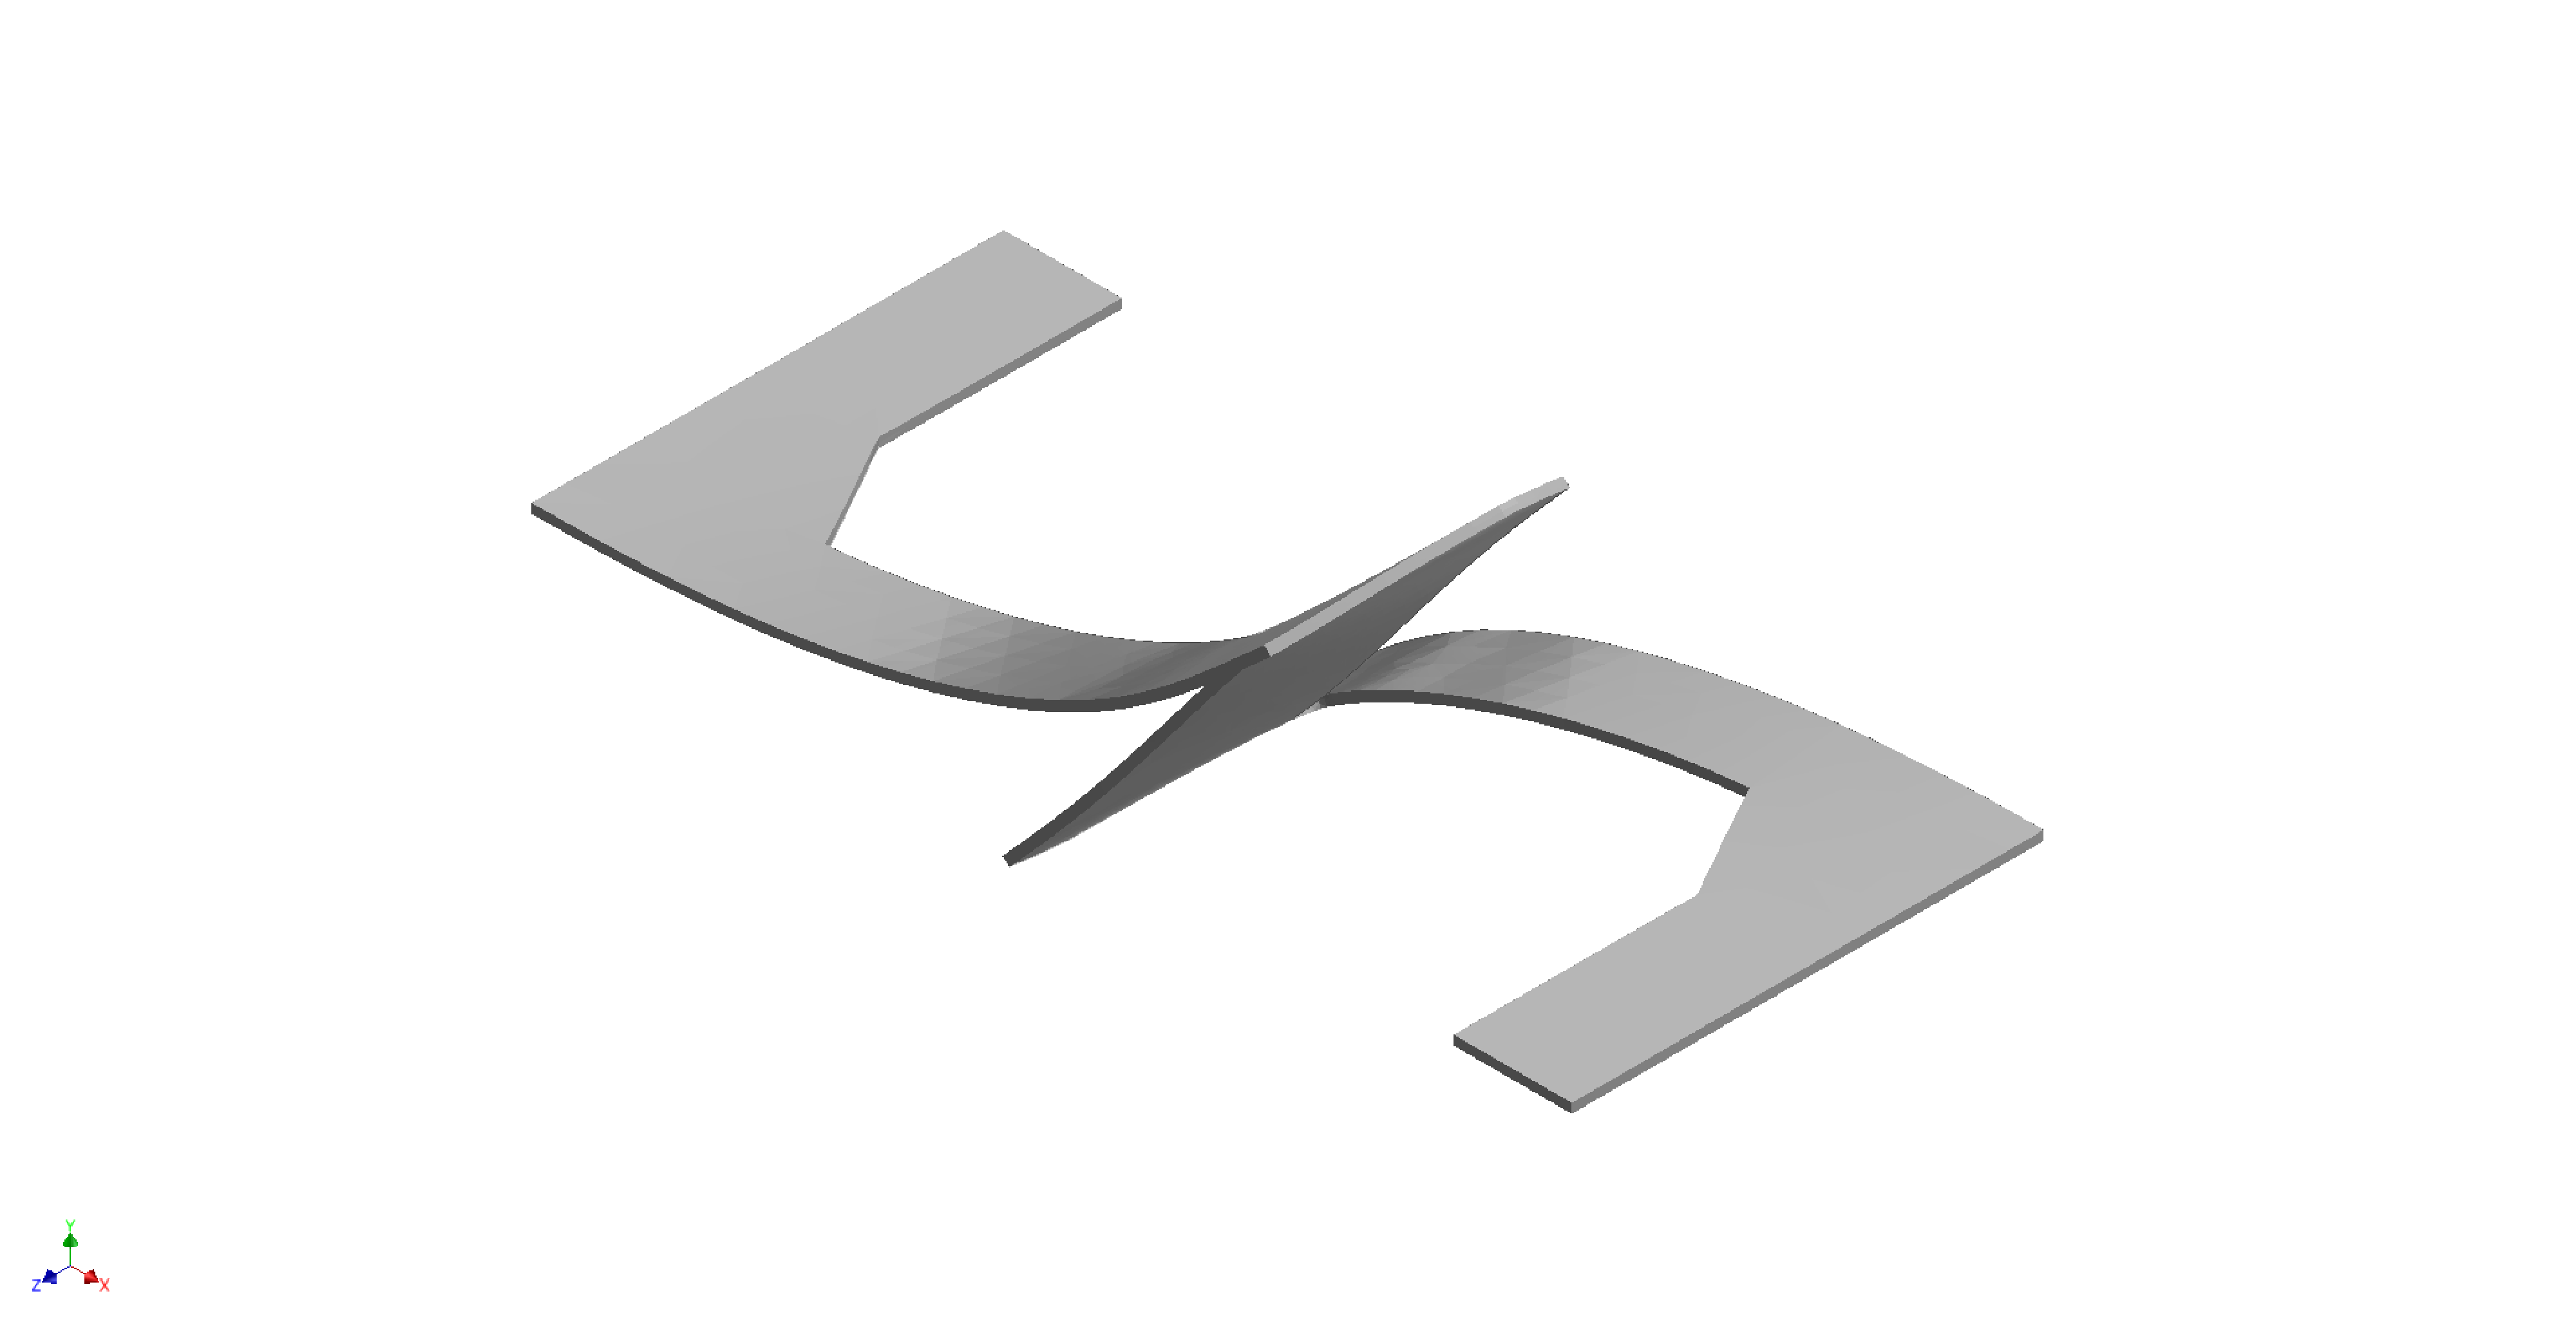
\includegraphics[width=0.75\textwidth,trim={5cm 0cm 5cm 5cm}, clip]{images/chap5/ohm-kiri-half-deformed-iso.pdf}
    };
    \node[anchor=south west,inner sep=0] (graph) at (0,0) {
        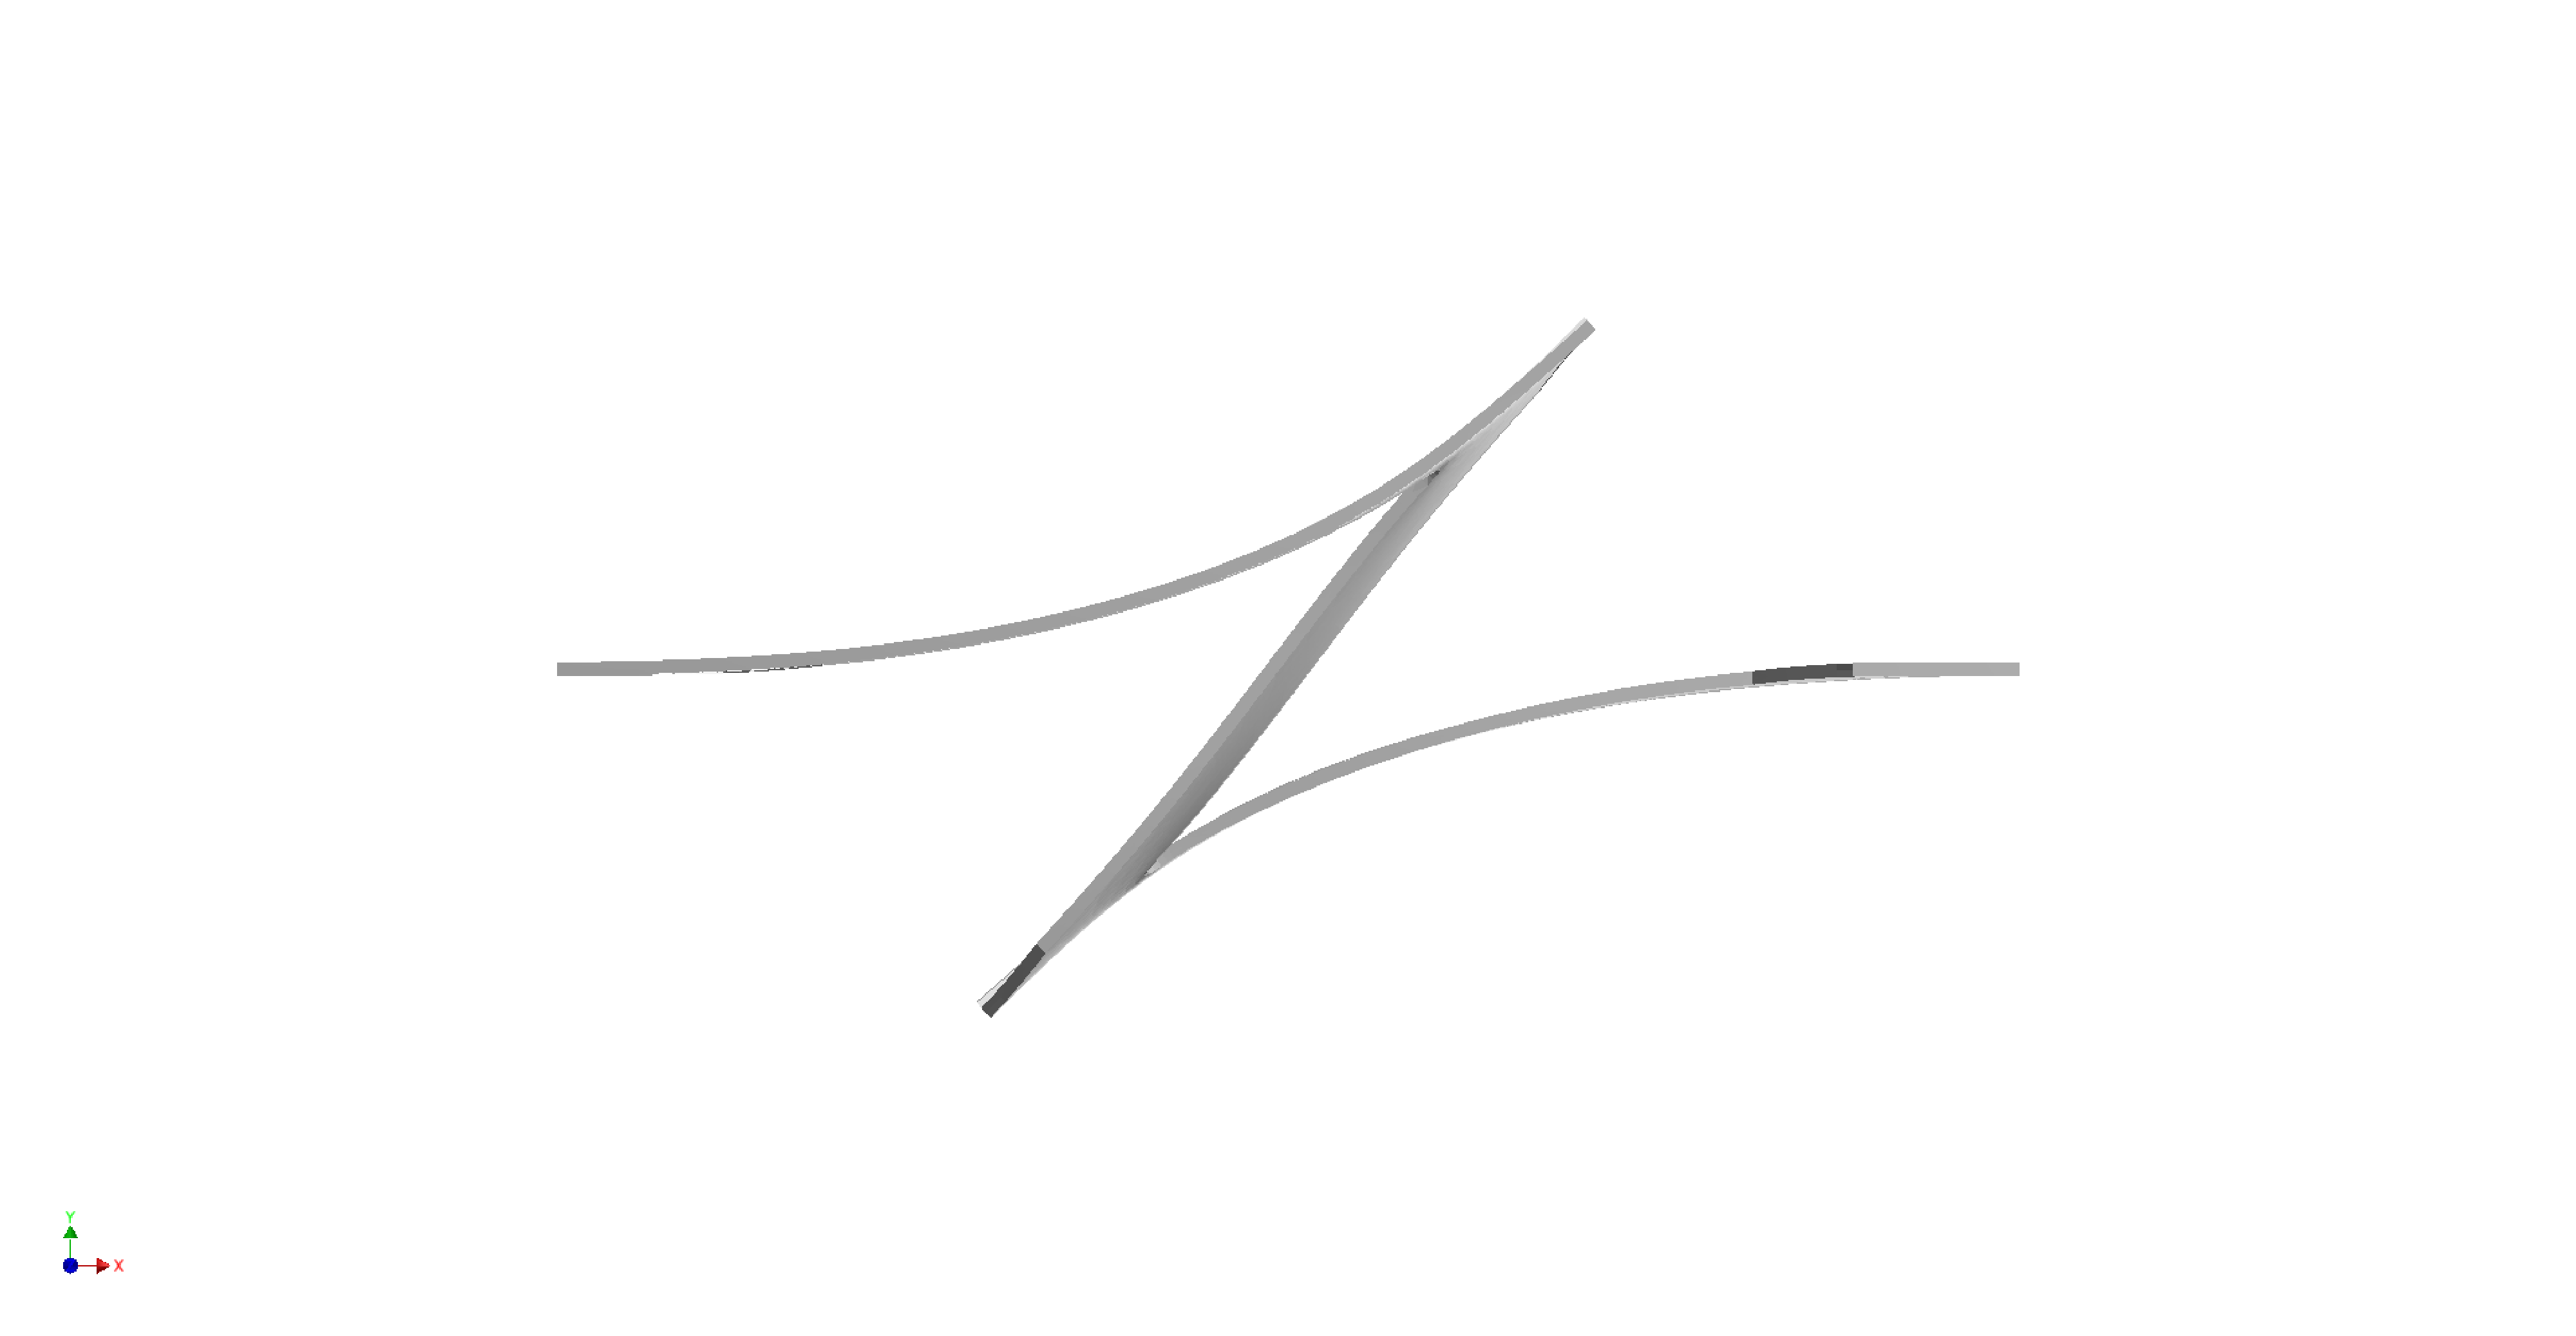
\includegraphics[width=0.75\textwidth,trim={5cm 5cm 5cm 5cm}, clip]{images/chap5/ohm-kiri-half-deformed-side.pdf}
    };
    \begin{scope}[x={(graph.south east)},y={(graph.north west)}]
        \draw[Circle-latex] (0.83,0.5) -- node[above] {$F$} (0.9,0.5);
        \draw[|-|] (0.75,0.45) -- node[below] {$\Delta x$} (0.83,0.45);
        \draw[-{Stealth[flex=1]}] (0.355,0.19) arc (110:350:6pt);
        \node (P) at (0.31,0.1) {$M$};
        \node[circle,fill,draw,scale=0.4] (Pc) at (0.5,0.5) {};
        \node (P) at (0.55,0.5) {$P$};
      % \draw[help lines,xstep=.05,ystep=.05] (0,0) grid (1,1);
      %   \foreach \x in {0,1,...,9} { \node [anchor=north] at (\x/10,0) {0.\x}; }
      %   \foreach \y in {0,1,...,9} { \node [anchor=east] at (0,\y/10) {0.\y}; }
    \end{scope}
\end{tikzpicture}
\end{document}
